\documentclass{jarticle}[2012/05/15]
\usepackage{graphicx}
\usepackage{misc}
\usepackage{listings,jlisting}
\begin{document}
\section{目的}
本実験の目的は、コンピュータビジョンのうち人間の視覚情報の処理を学ぶことである。
そのため、二次元平面画像に対する処理を学び、その基本を習得する。
\par
\section{理論}
\subsection{デジタル画像}
画像には、フィルム写真などで扱うアナログ画像と、
コンピュータで扱いやすいようにデジタル化したデジタル画像の2種類がある。
デジタル画像はアナログ画像の空間情報を画素と呼ばれる点に離散化し、
アナログ画像の濃淡情報を各画素に含まれる濃淡値として離散化したものである。
前者の処理を標本化、後者の処理を量子化という。
\par
\subsection{画像フォーマット}
デジタル画像をファイルに格納する際に、各情報をどのようにデータとして並べるか
またどのように圧縮するかなどのフォーマットは、現実には幾通りも存在する。
これはデジタル変換時に、利用環境・利用目的などにあわせてその都度決定する必要がある。
\par
\subsubsection{ppm、pgmフォーマット}
本実験で用いる画像フォーマットは、ppm,pgmフォーマットである
pgmはグレースケール画像データ、ppmは256階調カラー画像データを扱う形式である。
このフォーマットは単純に画素データを並べただけのもので、圧縮処理などはされていないため
基礎実験で用いるのは都合がいい。
\par
なお、本実験ではあらかじめ与えられた関数を通して画像データを処理するため、
ppm,pgmを直接操作することはない。
そのためppm,pgmフォーマットの詳細については省略する。
\par
\subsection{フォーマット同士の変換}
あるフォーマットの画像ファイルを別のフォーマットの画像ファイルへ変換することができる。
しかし、非可逆圧縮が施されていたり、変換後のフォーマットで扱える濃淡情報の量が
変換前のそれよりも少なかったりすると、変換時に情報の欠損が起きる。
\par
\subsection{画像処理}
デジタル画像処理では、一般に二次元画像をピクセルの二次元配列として扱う。本実験では「ポインタへのポインタ」型を二次元配列のように扱うことでこれを実現する。
\par
\subsection{濃度変換}
\subsubsection{濃度ヒストグラム}
濃度ヒストグラムとは、画像の濃度値とその分布を表すグラフである。
これを用いると、不鮮明な画像を鮮明に見せるための
濃度ヒストグラム変換と呼ばれる処理が行えるようになる。
\par
\subsubsection{濃度ヒストグラム変換}
ヒストグラムの分布を変えるような変換のこと。
本実験では、濃度値が値よりも高いものを白、そうでなければ黒とする2値化を行う。
これも濃度ヒストグラム変換の一種と言える。
\par
\subsubsection{コントラスト}
コントラストとは、画像中の濃淡情報の最大値から画像中の濃淡情報の最小値を引いた値である。
\par
コントラストが高いと画像は鮮明になる。
そのために用いる濃度ヒストグラム変換の手法をヒストグラムの部分拡張という。
\par
コントラストが低いと画像は不鮮明になる。
そのために用いる濃度ヒストグラム変換の手法をヒストグラムの平坦化という。
\par
本実験で用いる2値化は、コントラストを高めるための手法であり、ヒストグラムの部分拡張である。
\par
\subsubsection{2値化}
濃淡情報を0と1の2値画像に変換することを2値化(binarization)という。2値に分離するための境界はp-タイル法や判別分析法で求める。
\par
\subsubsection{p-タイル法}
取り出す図形の面積がある程度予測できるとき、
ヒストグラム上で全度数のうち明るい方からp[\%]のところを閾値とする方法
\par
\subsection{ラベリング}
2値画像において、画素が互いに連結して塊を形成しているものが図形成分となる。
画像中にはこのような図形成分が点在しているため、各々の連結成分に対して
異なった名前のラベルを与える処理をラベリングと呼ぶ
今回は、二値化画像の各々の画素の塊にそれぞれ対応する一意の名前(名前としての数値)を
与えたラベリング画像を別に生成し、このラベリング画像を用いて実験を行う。
\par
\subsubsection{図形融合}
二値化した画像は、多くの場合、小さな穴や点状図形を多く含んでいる。
この穴や点はノイズなので、図形の収縮と拡散を用いて除去する。
\par
今回用いる方法では1dotの近傍8dotに対して、収縮・拡散を行う。
\par
\subsection{輪郭線追跡}
図形の境界がつくる閉曲線を抽出する処理を輪郭線追跡という。
この処理の結果得られた閉曲線は画像の形状情報などを保存している。
これを形状解析やデータ圧縮の一つとして用いることができる。
\par
\subsection{認識システム}
画像の中身の内容がなんであるか知り、状況に応じて理解することを画像理解あるいは画像認識という。
この処理のための万能なアルゴリズムなどは存在しないため、目的に応じて
各画像処理のアルゴリズムを組み合わせ、システムを構成する必要があある。
\par
認識システムは、一般に「前処理」「特徴抽出」「認識判定」の3つの過程に分かれる。
\par
「前処理」で行うのは、ひずみ補正、画像の強調、画質改善などである。
\par
「特徴抽出」で行うのは、形状および濃淡に関する特徴量の抽出である。
\par
「認識判定」で行うのは、得られた特徴量を用いた認識のための判定である。
\par
\subsection{特徴量}
二値化した画像から抽出した図形は、
それそのものがi方向、j方向への特徴ベクトルを持っているが、その特徴ベクトルとは別に、
今回は図形の形状を表す特徴量として複雑度というスカラー値を用いる。
\par
\pagebreak

\section{方法}
あらかじめ用意されたライブラリに加えて、以下の自作関数を用いる。\par
{\scriptsize
\begin{lstlisting}
int DisplayColorImage (int **R, int **G, int **B);
int TranslateGrayScale(int **R, int **G, int **B, int **Y);
int MakeHistogram     (int **Y, int hist[256]);
int OutputHistogram   (int hist[256]);
int Percentile        (int **Y, int hist[256], double per);
int TranslateBoolScale(int **Y, int **F, int boader);
int remove_noise      (int **F, int loop);
int getLabeledImgLand (int **L, int label);
int printLabelingData (int **L, int label\_num);
int makeLabeled       (int **N, int **L, int label);
int DisplayLabeled    (int **N);
\end{lstlisting}
}
\subsection{実験1について}
実験1では、画像を処理する準備のために、画像ファイルをプログラムに取り込むう。同時にX Window Systemにウィンドウを表示する関数を実行する。
\subsection{実験2について}
実験1で表示したウィンドウに、実験1で取り込んだ画像ファイルをカラーで表示する。
\subsection{実験3-1,3-2について}
実験3-1では、実験2で表示させた画像を、グレースケールのものに変換してから表示させるようにする。実験3-2では実験3-1で表示させたグレースケール画像のヒストグラムを作成する。
\subsection{実験4について}
実験3-1で作ったグレースケール画像を白黒画像に変換する。
\subsection{実験5-1,5-2,5-3について}
実験5-1では実験4で作った白黒画像からノイズを取り除き、5つの図形にラベルをふって、それぞれの面積を求める。実験5-2ではラベルをふった図形それぞれに輪郭線追跡を行う。実験5-3では、それぞれの図形の輪郭線長と面積から特徴量を求める。

\section{用具}
本実験にはX11およびGCCを用いる。\par
GCCのコンパイルオプションには、「gcc -m32 Image.o Graphics.o 実験プログラム.c -lm -lX11 -ansi -std=c99 -Wall」\par
を用いる。\par
スクリーンショットはimportコマンドを用いてeps形式で保存する。\par
実験3-2のヒストグラムは、gnuplotを用いてeps形式で作成する。\par
\pagebreak

\section{結果}
\subsection{実験1}
デジカメで撮影したデジタル画像をプログラムに取り込んだ。図\ref{source}に、この画像をconvertコマンドでeps形式に変換したものを載せる。\par
\begin{figure}[htbp]
  \centering
  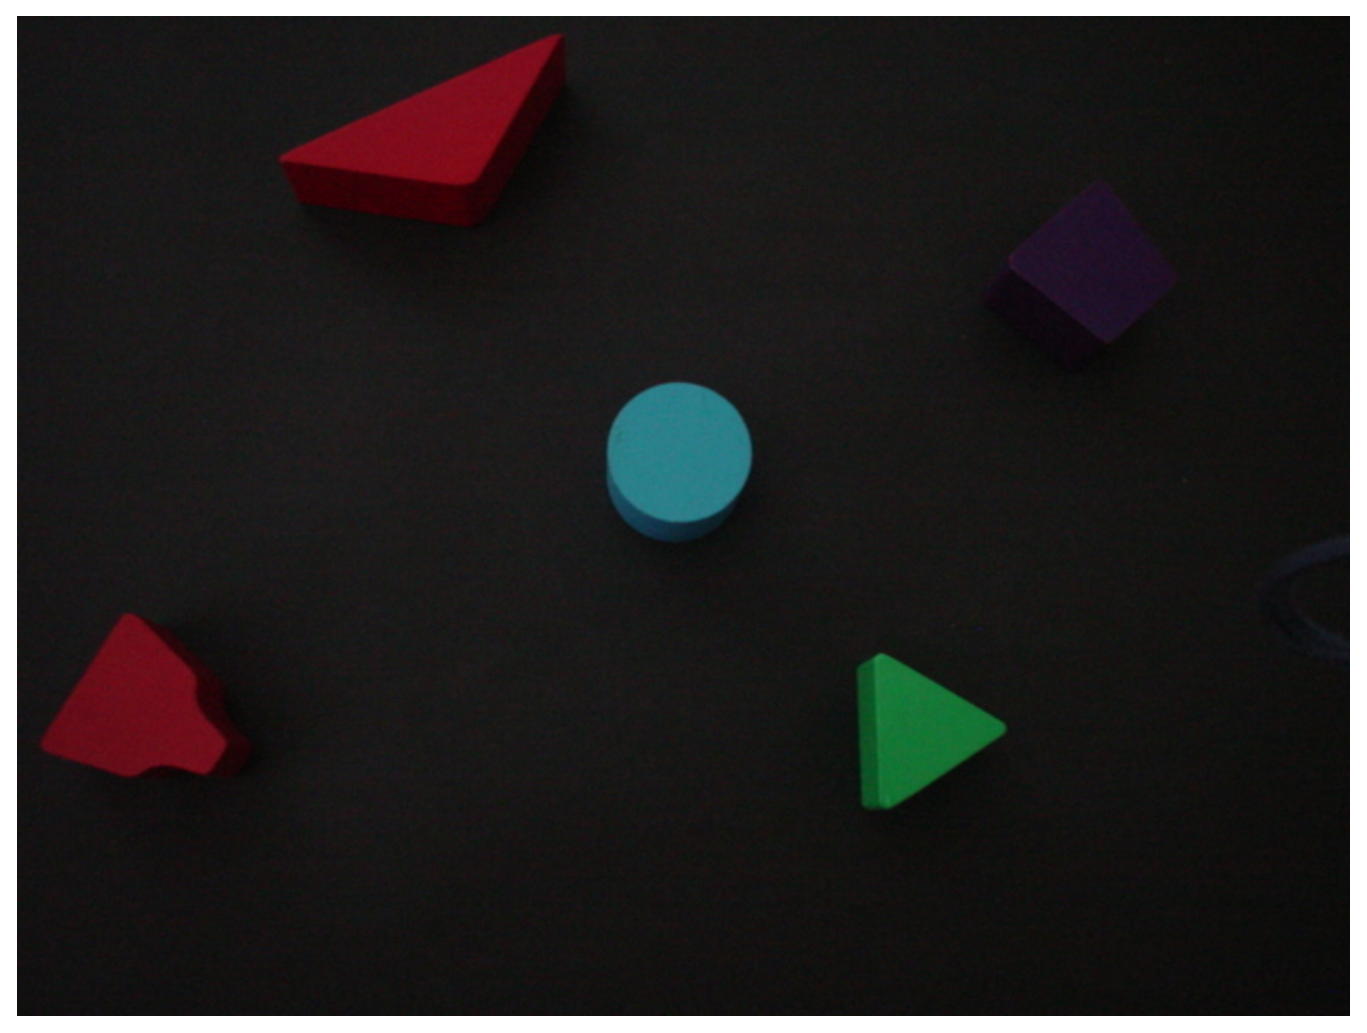
\includegraphics[width=8cm]{DSC00062.eps}
  \caption{デジタル画像} \label{source}
\end{figure}
実験1の実行結果を図\ref{kadai01}に示す。\par
\pagebreak
\begin{figure}[htbp]
  \centering
  \includegraphics[width=8cm]{kadai01.eps}
  \caption{実験1の結果} \label{kadai01}
\end{figure}
黒いウィンドウが現れた。\par
\pagebreak
\subsection{実験2}
実験2の実行結果を図\ref{kadai02}に示す。\par
\begin{figure}[htbp]
  \centering
  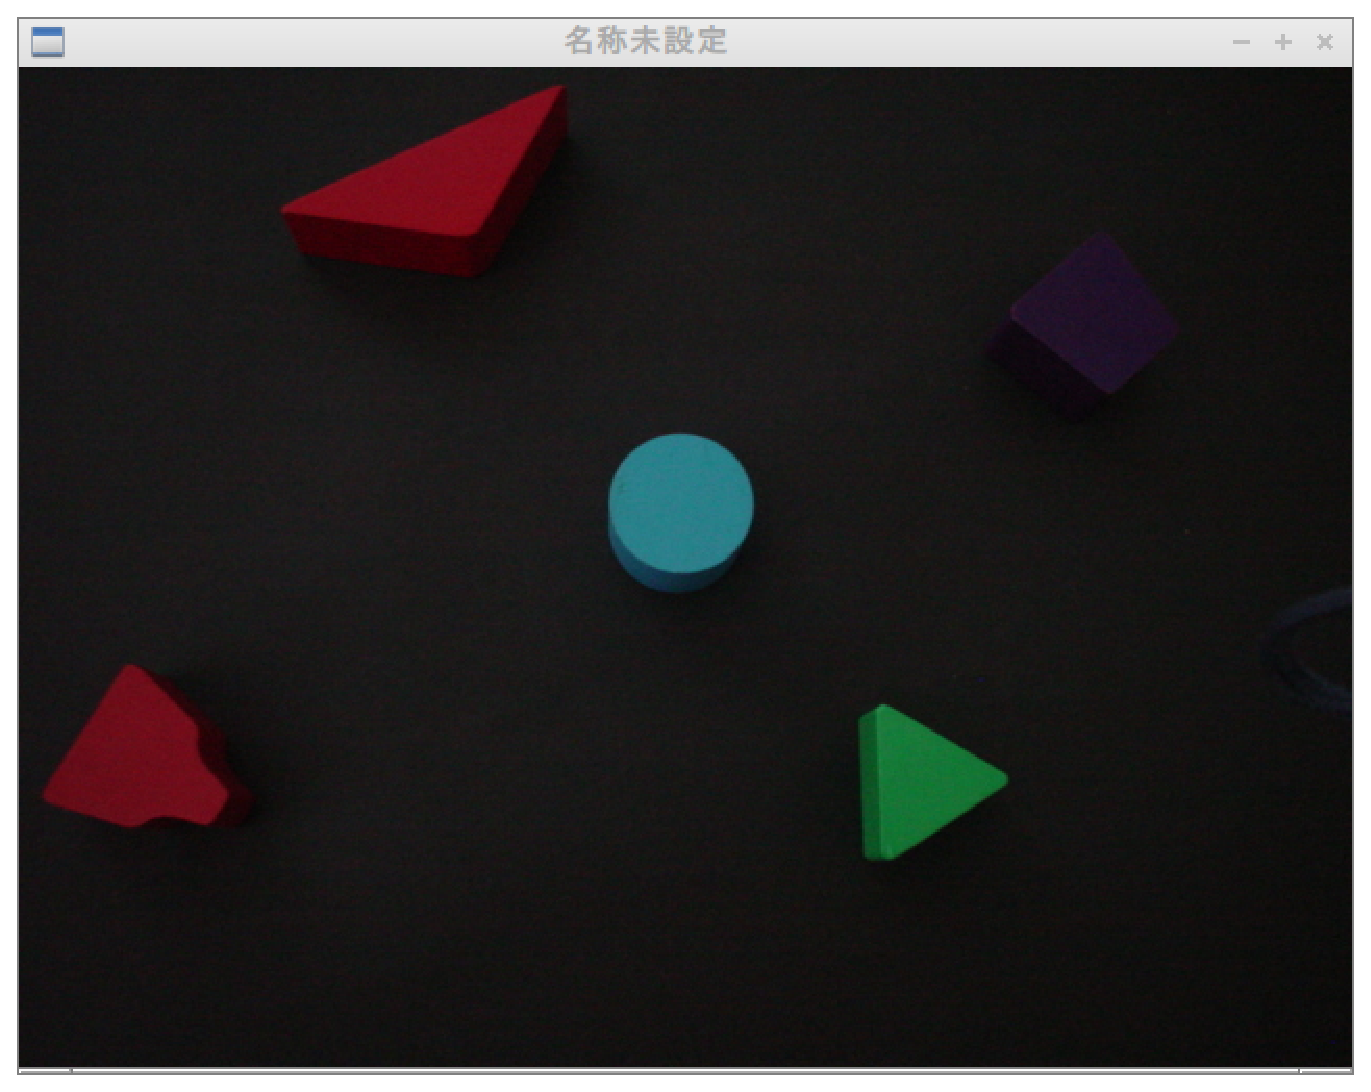
\includegraphics[width=8cm]{kadai02.eps}
  \caption{実験2の結果} \label{kadai02}
\end{figure}
カラー画像が現れた。
\pagebreak
\subsection{実験3-1}
実験3-1の実行結果を図\ref{kadai03-1}に示す。\par
\begin{figure}[htbp]
  \centering
  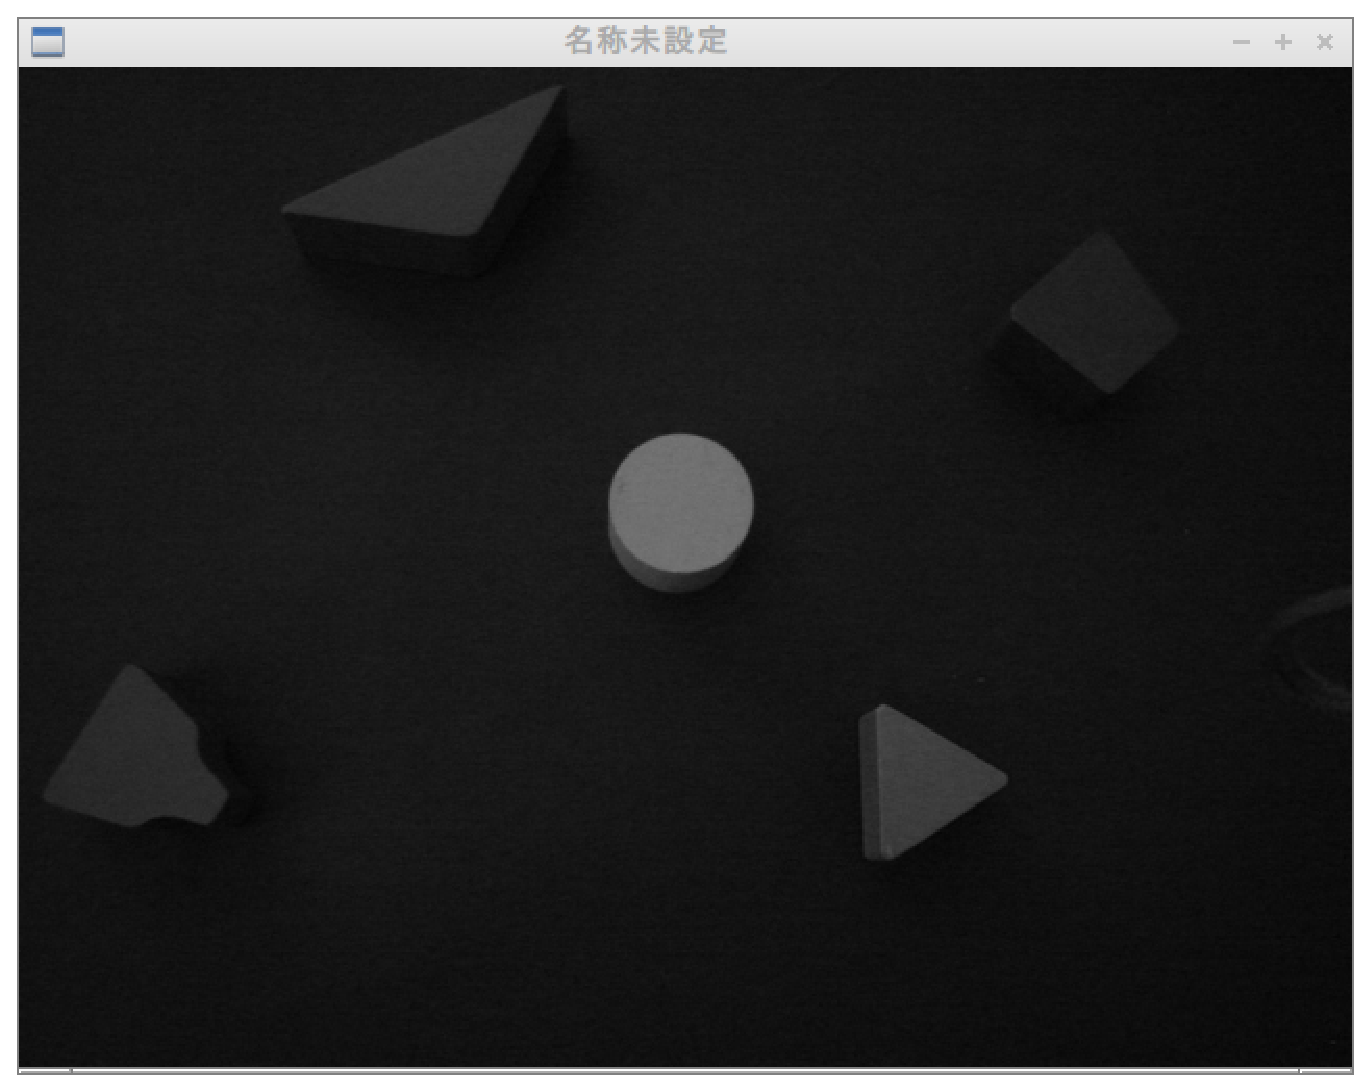
\includegraphics[width=8cm]{kadai03-1.eps}
  \caption{実験3-1の結果} \label{kadai03-1}
\end{figure}
グレースケール画像が得られた。
\pagebreak
\subsection{実験3-2}
実験3-2から得たヒストグラムを図\ref{hist}に示す。\par
\begin{figure}[htbp]
  \centering
  \includegraphics[width=8cm, angle = 270]{hist.ps}
  \caption{実験3-2の結果} \label{hist}
\end{figure}
ここでは-50~0、および256~300の値域も表示している。これはプログラムが正しければ理論上検出されないはずの値である。今回はプログラムにバグがないことを示すためにわざと「検出されるべき値域」の前後まで含めたこのヒストグラムを載せた。
\pagebreak
\subsection{実験4}
実験4の実行結果を図\ref{hist}に示す。\par
\begin{figure}[htbp]
  \centering
  \includegraphics[width=8cm]{kadai04.eps}
  \caption{実験4の結果} \label{kadai04}
\end{figure}
ノイズ混じりの二値画像が得られた。ノイズを除去後、これを実験5-1以降で使用することにした。\par
なお、ノイズ除去は実際には実験5-1以降のプログラムで行っており、本実験ではノイズ除去後の画像は表示していない。また、5-1以降でもそのような画像は出てこない。これは、ノイズが除去できたかどうかを「ラベルの数が5個」つまり「ラベルが図形の数と同じであるかどうか」をもとに判断したためである。
\pagebreak
\subsection{実験5-1}
実験5-1の実行結果を図\ref{kadai05-1}に示す。\par
\begin{figure}[h]
  \begin{center}
    \begin{tabular}{|p{8cm}|}\hline
label\_num=5
label=0,land =285482 \par
label=1,land =5387 \par
label=2,land =2745 \par
label=3,land =4855 \par
label=4,land =4757 \par
label=5,land =3974 \\ \hline
    \end{tabular}
    \caption{課題5-1の結果} \label{kadai05-1}
  \end{center}
\end{figure}
これより、ラベルが貼られた画像の数は5つであることが分かった。また、各々の面積も得られた。
\pagebreak
\subsection{実験5-2}
実験5-2の実行結果を図\ref{kadai05-2-1}から\ref{kadai05-2-5}に示す。\par
\begin{figure}[htbp]
  \centering
  \includegraphics[width=8cm]{kadai05-2-1.eps}
  \caption{実験5-2の結果1} \label{kadai05-2-1}
\end{figure}
\begin{figure}[htbp]
  \centering
  \includegraphics[width=8cm]{kadai05-2-2.eps}
  \caption{実験5-2の結果2} \label{kadai05-2-2}
\end{figure}
\begin{figure}[htbp]
  \centering
  \includegraphics[width=8cm]{kadai05-2-3.eps}
  \caption{実験5-2の結果3} \label{kadai05-2-3}
\end{figure}
\begin{figure}[htbp]
  \centering
  \includegraphics[width=8cm]{kadai05-2-4.eps}
  \caption{実験5-2の結果4} \label{kadai05-2-4}
\end{figure}
\begin{figure}[htbp]
  \centering
  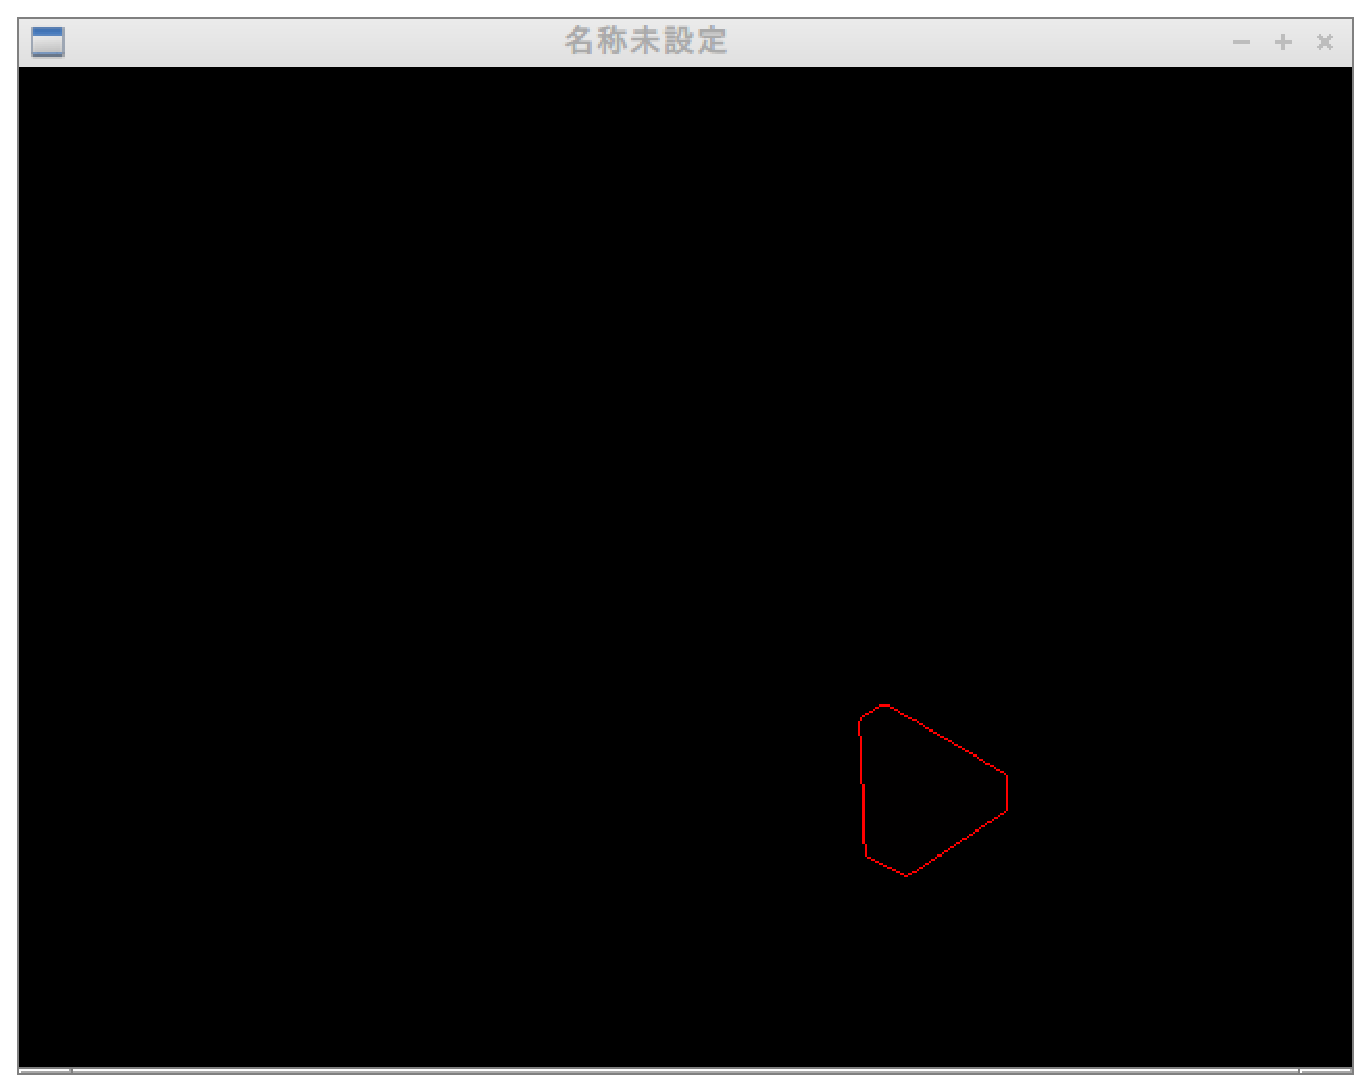
\includegraphics[width=8cm]{kadai05-2-5.eps}
  \caption{実験5-2の結果5} \label{kadai05-2-5}
\end{figure}
それぞれラベル付された画像が得られた。
\pagebreak
\subsection{実験5-3}
実験5-3の実行結果を図\ref{kadai05-3}に示す。\par
\begin{figure}[h]
  \begin{center}
    \begin{tabular}{|p{8cm}|}\hline
c[1]=18.4193
c[2]=33.667
c[3]=11.9631
c[4]=12.7215
c[5]=12.4016 \\ \hline
    \end{tabular}
    \caption{課題5-3の結果} \label{kadai05-3}
  \end{center}
\end{figure}
これより、各々のラベルの貼られた画像の特徴量Cが求まった。
\pagebreak

\pagebreak
\section{考察}
\subsection{実験1}
この実験からでは、Xが正しく扱えていることしか分からず、画像の処理については何も分からなかった。
\subsection{実験2}
画像が表示され、表示された画像が元の画像と同様であることから、正しく画像の取り込みと表示が行えたことがわかる。
\subsection{実験3-1}
ここで得たグレースケールは、赤:緑:青の比が1:1:2である。紫がのちの実験でうまく抽出できなかったために、青の比を多くした。
\subsection{実験3-2}
得られたヒストグラムから、全体的に暗めの画像であることが分かる。そのためパーセンタイル法でpの値を95\%程度とることにする。85\%とった場合でも同様の結果となった。
\subsection{実験4}
次の実験では一度この画像をグレースケールに変換後、ラベリングをする。そのためここでのノイズは除去する必要がある。近傍8dot(資料では4dotだったが、この数だとうまくいかなかったため変更した)を用いた拡大・縮小の場合、15回でちょうど余計なノイズがすべて消え、ラベルが5つ(画像内の対象物と同じ数)得られるようになった。
\subsection{実験5-1}
前節で適切にノイズ除去がされたことが、ラベルは全部で5つであり、また異常に小さな面積の画像もないことからわかる。画像内の対象物にラベルが貼られていることは次の節で確認する。
\subsection{実験5-2}
実際に対象物にラベルが貼られていることが分かる。紫の積み木の形がノイズ除去によって崩れてしまったのは、二値化時に紫の積み木の形が崩れてしまっており、それをノイズとして誤認識してしまったためである。
\subsection{実験5-3}
もっとも小さな値はC[3]であり、これが円であると認識した。結果、円柱は3つめの積み木であり、今回の場合はこの方法で正しく認識できた。
\section{感想}
あらかじめ用意された関数を使ったため、画像ファイルの中身が分かりにくく、画像情報の処理も中途半端にしか習得できなかったように思う。\par
\pagebreak
\section{ソースコード}
最後に、実験に使ったソースコードをまとめて載せる。\par
{\scriptsize
   \lstinputlisting[label=src:kadai01.c, caption=kadai01.c 課題1]{kadai01.c}
}
\pagebreak
{\scriptsize
   \lstinputlisting[label=src:kadai02.c, caption=kadai02.c 課題2]{kadai02.c}
}
\pagebreak
{\scriptsize
   \lstinputlisting[label=src:kadai03-1.c, caption=kadai03-1.c 課題3-1]{kadai03-1.c}
}
\pagebreak
{\scriptsize
   \lstinputlisting[label=src:kadai03-2.c, caption=kadai03-2.c 課題3-2]{kadai03-2.c}
}
\pagebreak
{\scriptsize
   \lstinputlisting[label=src:kadai04.c, caption=kadai04.c 課題4]{kadai04.c}
}
\pagebreak
{\scriptsize
   \lstinputlisting[label=src:kadai05-1.c, caption=kadai05-1.c 課題5-1]{kadai05-1.c}
}
\pagebreak
{\scriptsize
   \lstinputlisting[label=src:kadai05-2.c, caption=kadai05-2.c 課題5-2]{kadai05-2.c}
}
\pagebreak
{\scriptsize
   \lstinputlisting[label=src:kadai05-3.c, caption=kadai05-3.c 課題5-3]{kadai05-3.c}
}
\pagebreak
\end{document}